% THIS IS SIGPROC-SP.TEX - VERSION 3.1
% WORKS WITH V3.2SP OF ACM_PROC_ARTICLE-SP.CLS
% APRIL 2009
%
% It is an example file showing how to use the 'acm_proc_article-sp.cls' V3.2SP
% LaTeX2e document class file for Conference Proceedings submissions.
% ----------------------------------------------------------------------------------------------------------------
% This .tex file (and associated .cls V3.2SP) *DOES NOT* produce:
%       1) The Permission Statement
%       2) The Conference (location) Info information
%       3) The Copyright Line with ACM data
%       4) Page numbering
% ---------------------------------------------------------------------------------------------------------------
% It is an example which *does* use the .bib file (from which the .bbl file
% is produced).
% REMEMBER HOWEVER: After having produced the .bbl file,
% and prior to final submission,
% you need to 'insert'  your .bbl file into your source .tex file so as to provide
% ONE 'self-contained' source file.
%
% Questions regarding SIGS should be sent to
% Adrienne Griscti ---> griscti@acm.orghttps://www.overleaf.com/7267312825nsgbbwvhhrxchttps://www.overleaf.com/7267312825nsgbbwvhhrxc
%
% Questions/suggestions regarding the guidelines, .tex and .cls files, etc. to
% Gerald Murray ---> murray@hq.acm.org
%
% For tracking purposes - this is V3.1SP - APRIL 2009

\documentclass{edm_template}


\usepackage{tikz}
\usetikzlibrary{bayesnet}
\usetikzlibrary{arrows}
\usepackage{enumitem}
\usepackage{amsmath}
\usepackage{mathtools}

\DeclarePairedDelimiterX{\infdivx}[2]{(}{)}{%
  #1\;\delimsize\|\;#2%
}



\newcommand{\infdiv}{D_{KL}\infdivx}

% \usepackage[dvipsnames]{xcolor}

\providecommand{\am}[1]{{\color{blue} [AM: #1]}}
\providecommand{\nvg}[1]{{\color{red} [NG: #1]}}
\newcommand{\piech}[1]{{\color{purple}{[cjp: #1]}}}

\begin{document}

\title{Latent Variable Models of Enrollment for Course Planning and Understanding}

\numberofauthors{5} %  in this sample file, there are a *total*
% of EIGHT authors. SIX appear on the 'first-page' (for formatting
% reasons) and the remaining two appear in the \additionalauthors section.
%
\author{
% You can go ahead and credit any number of authors here,
% e.g. one 'row of three' or two rows (consisting of one row of three
% and a second row of one, two or three).
%
% The command \alignauthor (no curly braces needed) should
% precede each author name, affiliation/snail-mail address and
% e-mail address. Additionally, tag each line of
% affiliation/address with \affaddr, and tag the
% e-mail address with \email.
%
\alignauthor Nate Gruver \\
       \affaddr{Stanford University}\\
       \email{ngruver@cs.stanford.edu}
\alignauthor Ali Malik \\
       \affaddr{Stanford University}\\
       \email{malikali@cs.stanford.edu}
\alignauthor Brahm Capoor \\
       \affaddr{Stanford University}\\
       \email{brahm@cs.stanford.edu}
\and
\alignauthor Chris Piech\\
       \affaddr{Stanford University}\\
       \email{piech@cs.stanford.edu}
\alignauthor Mitchell Stevens\\
       \affaddr{Stanford University}\\
       \email{stevens4@stanford.edu}
\alignauthor Andreas Paepcke \\
       \affaddr{Stanford University}\\
       \email{paepcke@cs.stanford.edu}
}
% There's nothing stopping you putting the seventh, eighth, etc.
% author on the opening page (as the 'third row') but we ask,
% for aesthetic reasons that you place these 'additional authors'
% in the \additional authors block, viz.

% Just remember to make sure that the TOTAL number of authors
% is the number that will appear on the first page PLUS the
% number that will appear in the \additionalauthors section.

\maketitle
\begin{abstract}

Understanding large-scale patterns in student course enrollment is a problem of great interest to university administrators and educational researchers. Despite this, impactful decisions are often made without a good quantitative framework of the process underlying student choices. We propose a probabilistic approach to modelling course enrollment decisions, drawing inspiration from natural language processing and mixture models. We use 10 years of anonymised student transcripts from a large university to construct a Gaussian latent variable model that can learn the joint distribution over course enrollments. Such a model is generative in nature, allowing for a diverse set of inference queries while also being robust to data sparsity. We demonstrate the usefulness of this model in comparison to other approaches and show that it is able to capture underlying student interests that guide enrollment decisions. 
\end{abstract}

%% A category with the (minimum) three required fields
%\category{H.4}{Information Systems Applications}{Miscellaneous}
%%A category including the fourth, optional field follows...
%\category{D.2.8}{Software Engineering}{Metrics}[complexity measures, performance measures]
%
%\terms{Theory}

\keywords{Enrollment modeling, mixture models, Hidden Markov Model} % NOT required for Proceedings

\section{Introduction}

\begin{figure*}
    \centering
    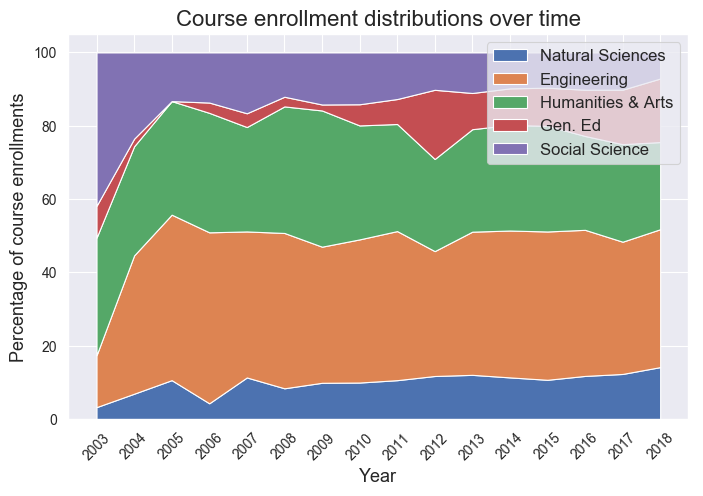
\includegraphics[scale=0.45]{figures/dists_over_time.png}
    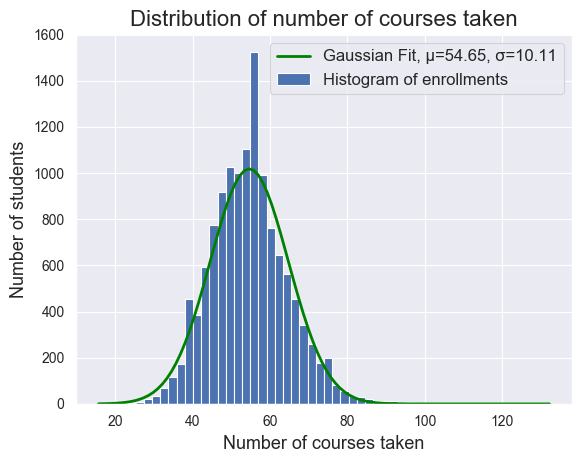
\includegraphics[scale=0.55]{figures/enrollment_dist.png}
    \caption{Top: A stacked area plot of enrolled courses per university sub-school per year. Bottom: A histogram of the number of courses taken by each individual student with a Gaussian fitting.}
    \label{fig:data_statistics}
\end{figure*}

Understanding the enrollment decisions of students in post-secondary institutions is central to the success of university administrators, researchers, and advisors. Despite this centrality, students and staff rely primarily on heuristics or complex mental models for the bulk of course planning. Although much work has been devoted to predicting course enrollments and collaborative filtering for course planning, few studies have attempted to replicate the robust framework experienced students hold within their head in a computational model. Such a model is not simply discriminative but is also capable of imagining counterfactuals, inferring intentions, or detecting anomalies in course planning.

To handle these more nuanced tasks, we propose a fully generative model of course enrollment. The distinguishing feature of a generative model is its ability to describe the full joint distribution over the feature space, in our case a student's binary-valued enrollments. This increased expressiveness makes it possible to calculate desired conditional or marginal probabilities \am{For ex. how likely is a student to take X conditioned on their past enrollments etc}.  Importantly, this property also makes it possible to draw joint samples from the model, the origin of the adjective ``generative". This capability means we can evaluate likely upcoming course choices based on the trained models' observations of all students' past choices.

The probabilistic nature of the generative model we propose here promises to serve \am{shows promise in serving} as a foundation for future course selection and student advising support facilities. For example, given an advising application built atop our model, advisers could evaluate how unusual a given student's proposed next-course choice would be, compared to paths that others have chosen in the past. Such insights could alert the advisor to pay extra attention to possible requirements conflicts, or the student's underestimation of workload.

A tool that we could imagine for students themselves would propose course choice paths towards a goal. The student could specify how much the suggestions should match `mainstream' choices, versus more unusual course tangents. While we have not written such high level applications, the model construction we propose here will enable their construction.

Somewhat more formally, these examples can be expressed in probabilistic terms as follows:

\begin{itemize}[noitemsep,topsep=0pt]
	\item A student prototyping their set of future enrollments based on common paths, i.e. queries of the form
	$$P(\text{Enrollment}_t \mid \text{Enrollment}_{1,..,t-1})$$ 
	\item An advisor wondering if their advisee is on track, i.e. queries of the form
	$$P(\text{Student's enrollment} \mid \text{All other student enrollments})$$
    \item An administrator trying to determine whether popular paths align with requirements, with queries of the form 
	$$\max_{C_i} P(\text{Clusters } C_i | \text{All enrollments})$$
\end{itemize}

These motivating examples represent a very small subset of the possible enrollment queries relevant to the operations of a university. These examples simply give a taste for how such questions can be framed in probabilistic language and then answered with the model presented here. 

\subsection{Prior Work}

Much of the prior work on enrollment modeling in the university setting is dedicated purely to predictive models, both of future course enrollment \cite{kardan2013prediction}\cite{nandeshwar2009enrollment}\cite{song1993new} and academic performance \cite{kovacic2010early}\cite{hlosta2017ouroboros}.
Perhaps the most compelling of these approaches is Kardan et al.'s use of a neural network trained on hand-selected features of a course and student to predict the probability of a future enrollment.  
Most state-of-the-art research in student decision modeling is now found in the study of massive open online courses (MOOCs). Studies of students in these course range in their focus from tracking student engagement to predicting future decisions and success. Gardner and Brooks \cite{Gardner2018StudentSP} provide a thorough overview of modern models for the problem, but we will mention two relevant approaches here. Balakrishnan and Coetzee use a Hidden Markov Model (HMM) to predict attrition in MOOCs by modeling the probability of a binary drop/no-drop decision per timestep \cite{balakrishnan2013predicting}. Similarly, Al-Shabandar et al. uses Gaussian Mixture Models (GMMs) to cluster MOOC students at each timestep, and thus identify clusters of students that are likely to withdraw  \cite{AlShabandar2018TheAO}. Both of these models are highly related to our approach in that they use graphical models to model student decisions. Their priority, however, is prediction of a simple binary outcome. In contrast, we seek to model the complex interactions of many courses jointly.

\piech{Include a paragraph on Bayesian Knowledge Tracing. This is 10/10 important for two reasons. One BKT is well known by the EDM and education community and some reveiwers are going to confuse the two and perhaps think you are solving a different problem. Here is an example paragraph. Not great writing but a start:}

\piech{Hidden Markov Models have historically been the ubiquitous solution to the ``Knowledge Tracing" task where students latent understanding is tracked as they provide answers to questions (CITE original BKT paper). Corbett & Anderson’s Bayesian Knowledge Tracing model
is now used to model student knowledge for computer programming, math and beyond (CITE a lot, see this paper for references: More Accurate Student Modeling through Contextual Estimation of Slip and Guess Probabilities in Bayesian Knowledge Tracing). 
Our work is different in two ways (1) we are using bayesian models to track students across courses using course performance as inputs and (2) We use a different type of Hidden Markov Model that can do XYZ (explain the delta from vanilla HMM to your GMM). }

Another related body of work is course recommender systems, which often leverage enrollment prediction as a subsystem, along with more sophisticated models of intention. Khorasani et al create a fully-observed Markov model of course enrollment sequences, estimating the probability of taking a course after others via maximum likelihood estimation (MLE)~\cite{Khorasani2016AMC}. Their use of a sequential probabilistic model parallels ours, but our use of latent variables gives us the added benefit of robustness to cases in which maximum likelihood is weak---namely when there are few examples of some enrollment patterns or when the number of variables being modeled jointly grows large. Jiang et al. achieve a similar level of sophistication in their neural-network based course recommender system~\cite{Jiang2018GoalbasedCR}, which uses predictions of grade outcomes to create custom course recommendations. Instead of a fully probabilistic model, they employ a recurrent neural network (RNN) using past semesters as input to the predictions. Though this model yields compelling results, it is not capable of the broad range of queries possible with our model. The most immediate limitation is in its ability to reason backwards in time, estimating probabilities on earlier states given future ones. In general, deep learning algorithms also often suffer from over-fitting when learning small datasets \am{Maybe cite}. 

A final significant branch of enrollment modeling research in the university setting is not related to prediction at all, but instead focuses on clustering courses for the purpose of understanding the semantic landscape of a university. These studies relate to the work here in so far as they seek to discover relationships between courses. Some authors focus on clustering courses~\cite{Motz2018FindingTI}\cite{Pardos2018AMO} while others focus instead on students~\cite{Zeidenberg2011TheCO}\cite{Slim2016TheIO}. The two common approaches for clustering courses are latent variable models like Latent Dirichlet Allocation (LDA) used by Motz et al. and Recurrent Neural Networks (RNNs) as used by Pardos et al. In our work, we directly consider both deep learning and simpler latent variable models like LDA and use these models as comparisons for our model. Among the authors that focus more directly on clustering students, Zeidenberg primarily defines distance metrics~\cite{Zeidenberg2011TheCO} over students, and Slim et al. present feature extraction approaches using graph operations~\cite{Slim2016TheIO}. 

Another notable growing field of research revolves around treating co-enrollments as a network and extracting graph-theoretic properties for feature learning~\cite{gardner2018coenrollment}\cite{Wang2017AnalyzingCC}. We considered related approaches in this work and ultimately found them less helpful than simple encoding schemes.

The primary limitation of the prior work is a lack of flexibility. Strong predictive models can be trained, but they are discriminative instead of generative and thus lack the ability to answer nuanced inference queries. Adopting the more general probabilistic approach presented here opens the door for a much more diverse set of analyses within a shared statistical framework.

\section{Background \& Models}

There is a rich history of using probabilistic graphical models (PGMs) in the study of natural language. Conveniently, natural language processing (NLP) shares many characteristics with the enrollment modeling task at hand. First, both concern categorical and sequentially structured data. Second, both enrollments and natural language tokens can be understood as the observable counterpoints to mostly unobserved semantic intentions. Noting these similarities, it is apt to use models that have also found success in NLP---here modeling enrollments as analogues of natural language tokens and students as the documents comprising these enrollments. In particular, we employ latent variable models precisely for their ability to capture the underlying typography of students and the sequential nature of their enrollments. 

\subsection{Latent Variable Models}
\label{section:latent-variable-models}

Latent variable models are a subclass of PGMs in which some variables are never observed in training data and are thus ``latent". These models are typically computationally demanding because of the marginalization required to calculate probabilities without fixed assignments to these hidden variables. They also, however, allow us to learn potentially complex structure in data without supervision. 

Among the simplest and most commonly used latent variable models is Latent Dirichlet allocation (LDA)---used for clustering of natural language documents. In this model, a latent variable captures the topics that could be present in a document, and words are drawn from a distribution conditioned on this topic. A slightly simplified version of LDA could be described with the generative process below:
\begin{align*}
\theta &\sim \text{Dir}(\alpha) \\
\text{ topic } z_i &\sim \text{Multinomial}(\theta) \\
\text{ word } w \mid z_i &\sim \text{Multinomial}(\beta) \\ 	
\end{align*}
\vspace{-11mm}

\am{The above probably needs to be explained in english. Also we don't cite LDA}

One obvious drawback of this model is its assumption that words are drawn independently given the selected topics. In the case of course enrollments this is problematic for at least two reasons: first because enrollment decisions often affect one another, and second because the number of courses taken by students in any given year is stochastic and dependent on the courses taken. It is easier to capture these two facets of the data if we can model enrollments jointly.

Take $X_i$ to be set of enrollments for a student $i$ with 
$$X_{ij} = 
\begin{cases}
\,\,1 & $student $ i $ took class $ j \\
-1 & $otherwise$
\end{cases}
$$
Any joint probability distribution over all discrete combinations of $X_i \in \{-1,1\}^m$ would require $2^m - 1$ parameters to specify and is thus impractical. We can, however, relax the discrete problem to a real-valued vector space with $\bar{X}_i \in \mathbb{R}^m$ and $X_{ij} = \text{sign}(\bar{X}_{ij})$. With this alternative encoding of enrollments we can take advantage of real-valued distributions with much smaller parameters spaces. 

The Gaussian Mixture Model (GMM) is an archetypal latent variable model for real-valued data. Much like LDA, there is a latent variable intended to capture semantics and an emission model specifying the probability of the observed features conditioned on the latent variable. In particular, we can describe a GMM by generative process below:
\begin{align*}
h_i &\sim \text{Multinomial}(\theta) \\
\bar{X} \mid h_i &\sim \mathcal{N}(\mu_i, \Sigma_i) \\
\end{align*}
\vspace{-11mm}

A graphical representation of the mixture model with hidden categorical variable $h$ and observed enrollment vector $\bar{X}$ is also shown in Figure \ref{fig:mixture_model}. At face value it might seem odd to model enrollments as distributed according to a Gaussian, but there are at least two convincing ways to view this choice. First, we can note that a Gaussian is simply encoding an assumption of smoothness around a modal assignment. In our case that will be the modal set of enrollments corresponding to a certain cluster of students. Smoothness will describe the way that most students in this cluster will be drawn from the same mold with small variations being most common. Another convincing way to view the choice of a Gaussian follows the Central Limit Theorem, which shows that the averaged stochastic individual choices of a student tends towards a multivariate normal in the limit.

\begin{figure}
	\centering
	\tikz{
	% nodes
	\node[obs] (X0) {$X_i$};%
	\node[latent,above=of X0] (h0) {$h_i$}; %
	\node[latent,rectangle,left=of h0] (theta0) {$\theta$}; %
	\node[latent,rectangle,left=of X0] (params0) {$\mu_k, \Sigma_k$}; %
	
	\node[latent,rectangle,right=1.5cm of X0] (params1) {$\mu_k, \Sigma_k$}; %
  	\node[latent,rectangle,right=1.5cm of h0] (theta1) {$\theta, \phi$}; %
	
	\node[obs,right=of params1] (X1) {$X^t_i$};%
	\node[latent,above=of X1] (h1) {$h^t_i$}; %
	
	% plate
	\plate [inner sep=.25cm,yshift=.2cm] {plate0} {(X0)(h0)} {$N$}; %
	\plate [inner sep=.25cm,yshift=.2cm] {plate1} {(X1)(h1)} {$N$}; %
	\plate [inner sep=.25cm,yshift=.2cm] {plate2} {(params0)} {$K$}; %
	\plate [inner sep=.25cm,yshift=.2cm] {plate3} {(params1)} {$K$}; %
	
	% edges
	\edge {h0} {X0}  
	\edge {theta0} {h0}
	\edge {params0} {X0}
	
	\edge {h1} {X1}
    \edge {theta1} {h1}
	\edge {params1} {X1}
	\draw (h1) edge[loop above] node {} (h1)}
	\caption{\label{fig:mixture_model} Graphical representation of mixture model (left) and hidden Markov model (right) using plate notation}
\end{figure}

\subsection{Contextual Mixture Model}

Hidden Markov Models (HMMs) are a common extension of the stationary mixture models to sequential data (Figure~\ref{fig:mixture_model}). In these models the single latent variable is replaced with a Markov chain \am{of hidden states, with future states influenced by the previous one}. This model is naturally recursive, a property that is extremely useful when modeling processes that are positive recurrent. However, as enrollments are for the most part directional \am{What does this mean?} and returning to previous states is unlikely, we prefer a model that is strictly time-dependent, or as we shall call it here ``contextual". In general any ``Contextual" Mixture Model (CMM) can be expressed using a Hidden Markov model, but enforcing this structure allows us to incorporate priors that significantly improve the chances of training a plausible model.

For a general HMM with Gaussian emission probabilities, we have 
\begin{align*}
h^0 &\sim \text{Multinomial}(\theta) \\    
h^{t+1} \mid h^{t} &\sim \text{Multinomial}(\phi) \\
x^{t} \mid h_i^{t} &\sim \mathcal{N}(\mu_i, \Sigma_i)
\end{align*}
In contrast, for a CMM we have 
\begin{align*}
h^0 &\sim \text{Multinomial}(\theta) \\    
h^{t+1} \mid h^{t} &\sim \text{Multinomial}(\phi^t) \\
x^{t} \mid h_i^{t} &\sim \mathcal{N}(\mu^t_i, \Sigma^t_i)
\end{align*}
Note that the parameters of the transition and emission distributions are different for each timestep. Figure~\ref{fig:contextual_mixture_model} shows a diagram of our proposed model in plate notation.

\begin{figure}
    \centering
	\tikz{
	% nodes
	\node[obs] (X0) {$X^0_i$};%
	\node[latent,above=of X0] (h0) {$h^0_i$}; %
	\node[latent,rectangle,above=of h0] (theta0) {$\theta^0$}; %
	\node[latent,rectangle,below=of X0] (params0) {$\mu^0, \Sigma^0$}; %	
	
	\node[obs,right=of X0] (X1) {$X^1_i$};%
	\node[latent,above=of X1] (h1) {$h^1_i$}; %
	\node[latent,rectangle,above=of h1] (theta1) {$\theta^1,\phi^1$}; %
	\node[latent,rectangle,below=of X1] (params1) {$\mu^1, \Sigma^1$}; %	
	
	\node[obs,right=of X1] (X2) {$X^2_i$};%
	\node[latent,above=of X2] (h2) {$h^2_i$}; %
	\node[latent,rectangle,above=of h2] (theta2) {$\theta^2,\phi^2$}; %
	\node[latent,rectangle,below=of X2] (params2) {$\mu^2, \Sigma^2$}; %	

	\node[obs,right=of X2] (X3) {$X^3_i$};%
	\node[latent,above=of X3] (h3) {$h^3_i$}; %
	\node[latent,rectangle,above=of h3] (theta3) {$\theta^3,\phi^3$}; %
	\node[latent,rectangle,below=of X3] (params3) {$\mu^3, \Sigma^3$}; %	
	
	% plate
	\plate [inner sep=.25cm,yshift=.2cm] {plate0} {(X0)(X1)(X2)(X3)(h0)(h1)(h2)(h3)} {$N$}; %
 	\plate [inner sep=.25cm,yshift=.2cm] {plate1} {(params0)(params1)(params2)(params3)} {$K$}; %
	
	% edges 
	\edge {theta0} {h0}
	\edge {h0} {X0}
	\edge {params0} {X0}
	
	\edge {theta1} {h1}
	\edge {h0} {h1}
	\edge {h1} {X1}
	\edge {params1} {X1}
	
	\edge {theta2} {h2}
	\edge {h1} {h2}
	\edge {h2} {X2}
	\edge {params2} {X2}
	
	\edge {theta3} {h3}
	\edge {h2} {h3}
	\edge {h3} {X3}
	\edge {params3} {X3}}
	
	\caption{\label{fig:contextual_mixture_model} Graphical representation of contextual mixture model using plate notation}
\end{figure}

For any contextual mixture model over $T$ timesteps we have
\begin{align*}
ll(\mathcal{D}, \, &h^{0:T} ; \, \theta,\phi^{1:T},\mu^{1:T},\Sigma^{1:T}) \, = \\
&\sum_{i=1}^N \log P(h^0) + \sum_{t=1}^T \log P(X^t_i \mid h^t) + \log P(h^t \mid h^{t-1})
\end{align*}
Thus $ll(\mathcal{D})$, the log-likelihood of the data, can be obtained by marginalization of the hidden variables. Training of the model can be performed with Expectation-Maximization (EM) via an algorithm analogous to the Baum-Welch algorithm (parameter updates given in the appendix) or via gradient descent on the negative log-likelihood \am{Cite}. In this work we use a combination of EM and gradient descent, taking advantage of the strong initial gains made by EM before using the online process of Stochastic Gradient Descent. 

In order to make learning $\Sigma^t_i$ possible given the constraint of positive semi-definiteness, we parametrize the multivariate normals by $\mu_i^t$ and the Cholesky decomposition, $T$, of each precision matrix, $(\Sigma^t_i)^{-1}$, with $TT^\top = (\Sigma^t_i)^{-1}$. Samples can thus be drawn from each Gaussian via 
$$\bar{X} = \mu + T^{-\top} z$$ 
for $z \in \mathbb{R}^m$ drawn from $\mathcal{N}(0,I)$. 

Further, the convenient properties of Gaussian allow us to write tractable forms for common inference queries. Take for instance the query
$$P(\text{Takes course } i \text{ in year } t \mid \text{Took courses } j,k \text { in years } t-1,t+1)$$
The probability of each assignment to hidden state $t$ can be calculated by inference on the Markov chain given evidence courses, $E$. This is made tractable with a forward and backward pass as in the Baum-Welch algorithm. When calculating $P(h_{t'} \mid E)$, we can take advantage of the fact that $P(E_{t'} \mid h_{t'})$, the marginal probability of the evidence variables at time $t'$ will simply be $\mathcal{N}(\bar{X}_E;\mu_E,\Sigma_E)$ where $E$ denotes the indices corresponding to evidence variables. 

The probability of the individual course $i$ can then be calculated as 
\begin{align*}
\sum_h \int_0^{\infty} \mathcal{N}(\bar{X_i} \mid h; \mu_i,&\Sigma_{ii}) p(h \mid E) d\bar{X} = \\
&\sum_h (1 - \Phi(0 \mid h ; \mu_i,\Sigma_{ii})) p(h \mid E)
\end{align*}
If we are additionally conditioning on evidence from the year $t$ itself we first compute the parameters of the conditional normal, $\mathcal{N}(\mu^*, \Sigma^*)$, with 
\begin{align*}
\mu^* &= \mu_{N} + \Sigma_{N E} \Sigma_{E E}^{-1} (x_E - \mu_E) \\
\Sigma^* &= \Sigma_{N N} - \Sigma_{N E} \Sigma_{E E} \Sigma_{E N}
\end{align*}
where $E$ denotes the indices corresponding to evidence variables and $N$ the remaining indices. The probability calculation can then be made via the CDF of the marginal distribution as above swapping in the conditional $\mu_i^*, \Sigma_{ii}^*$.

One could rightly point out that HMM-style models have been largely phased-out by models built around Recurrent Neural Networks in state-of-the-art NLP settings and thus question why we choose a simpler generative model. Our choice was made with at least two important factors in mind. First, in the current setting in which we seek a model for understanding as much as optimal prediction of enrollments \am{this reads weirdly}, the small discrete latent space of our model offers highly interpretable representations compared with the continuous latent vector space of neural architecture. Second, for the applications we described in the introduction, a fully generative model is necessary. Only highly complex variational neural architectures are capable of all the inference queries we describe, and these models can often suffer from suboptimal inference when there is overfitting of the decoder network. As we are operating on relatively small datasets, this shortcoming is especially relevant.

\section{Data}

\am{This section needs a transition. We go straight from maths into data... We should have an experiments section before this and have data be a subsection maybe. Related: we should present an overview of the sections in the intro}

We use 18 years of course enrollment data from a large private university in the United States. The data was given in the form of 2.15 million anonymized enrollment records with fields for course name and student major. Importantly, this dataset included not only the enrollment data of full-time students but also part-time and summer school students who were removed before the model was trained. 

\am{Preprocessing steps}

Figure~\ref{fig:data_statistics} shows two basic visualizations of the data after these pre-processing steps \am{after what preprocessing steps?}. There are at least two notable takeaways from these plots. First, despite rapid changes in the distribution of sub-school\footnote{These are the broadest partitions of the university which ungraduate commonly take classes in.} enrollments in the first few years of the data, the proportion of enrollments in each school remains relatively stable through most of the data. We use this fact to aggregate over time without explicitly modeling the changes in enrollments patterns. Second, the fact that the number of courses taken can be fit well with a Gaussian shows that enrollment patterns are not intensely multi-modal and thus the assumptions of probabilistic model are very plausible.

In order to learn the parameters of our model, we created training data by aggregating student enrollments per-year and encoding them in the $-1/1$ scheme described in Section~\ref{section:latent-variable-models}. With this data we could train a sequential model of enrollments \textit{per-degree} \am{per-degree sounds graph theoretic. maybe per major?}. This step was not strictly necessary and degree could have been modeled latently, but as most of our motivating queries are made at the level of department, this did not feel like a sacrifice. The results presented here are from models of the 4-year undergraduate degree programs in Computer Science, Math, and Philosophy, which were most familiar to the authors. 

As most of the resulting matrices were of dimension $(n,m)$ with $m > 10^3$, we additionally performed dimensionality reduction by removing classes that were enrolled in less than 10 times by all students of a major over the entire time period. This step also acted as a form of denoising as these enrollments tended to be less correlated with the others. 

\section{Model Selection and Verification}

\subsection{Numerical Metrics}

Because our model approximates a discrete distribution with a real-valued one, validation with log-likelihood becomes difficult--as the hold-out data represents an extremely collapsed subset of the model's support. This leads to often monotonically decreasing standard log-likelihood metrics. Here we present an alternative metric that can be used to gauge progress during training and compare models when selecting their final parameters. 

We can avoid the detrimental effects of the real-valued relaxation by directly comparing samples from our model, which are discretized, with hold-out data. More specifically, we can compare the empirical enrollment distributions in samples from our model and the hold-outs. Let $p^t_j$ be the probability that class $j$ is taken by any given student in the test data, and $p^s_j$ be the corresponding probability in the samples. We take as our error, $E(p^t,p^s)$ with 
\begin{align*}
 E(p^t,p^s) 
 &= \sum_j \infdiv{p^t_j} {p^s_j} \\
 &= - \sum_j p^t_j \log \left( \frac{p^s_j}{p^t_j} \right) + (1 - p^t_j) \log \left(\frac{1-p^s_j}{1 - p^t_j} \right)
\end{align*}
This is precisely the KL divergence between the mean field approximations of the two distributions. In this context, however, it is simply a metric we can use to estimate of the distance between the distribution of our model and the distribution of the data. 

When training a model, we can use this metric to determine hidden state size. This decision is inherently a tradeoff between accuracy and computational efficiency. Increasing the size of the hidden states increases the ability of the model to fit the data  \piech{what about overfitting? This would be an alarming sentence if I were a reviewer. I get what you mean, but I started reading in this section (most reviewers make sure a paper has results before they dive deep in)}  but the time required to perform inference scales quadraticly.Figure~\ref{fig:kl_plot} shows a plot of the error as a function of hidden state size for our proposed model as well two comparison models. By looking at the ``elbow'' of the plot, we can identify a reasonable hidden state size that balances accurate modeling of the distribution with computation complexity.

Figure~\ref{fig:kl_plot} also shows the comparative performance of our model relative to lower and higher complexity generative models. The latent categorical model is simply an LDA model with an additional inference step that improves sampling. The variational autoencoder (VAE) curve is a simple feedforward decoder trained on reconstruction loss. It is easy to observe that our model strikes the perfect balance of expressiveness given the size of our data in this investigation. The simple LDA model with its many simplifying assumptions is unable to fit the data well for any number of hidden states and the highly expressive VAE quickly overfits and thus performs poorly on the hold-out set. 

\begin{figure}[h]
    \centering
    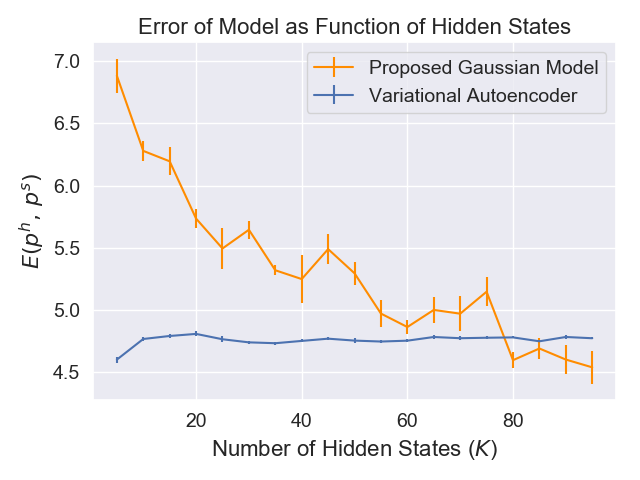
\includegraphics[scale=0.5]{figures/error_vs_hidden_states.png}
    \caption{A plot of the error for our GMM-based model: two comparison models as a function of hidden state size. The parameter $K$ in the discrete models (LDA and ours) is simply the number of possible hidden state values, whereas it is the dimension of the hidden vector space in the VAE.}
    \label{fig:kl_plot}
\end{figure}

\subsection{Visualizing Hidden Variables}

Beyond using the loss function defined with KL divergence, we can also examine the hidden states of a trained model to validate the learning process. In particular, we can look to see that the hidden space captures semantically meaningful categories. Figure~\ref{fig:gmm_clusters} shows a visualization for the model trained on CS majors. The clusters in the grid correspond to known departmental requirements connected to concentration within the major and color shows the most likely latent state assigned by the model. From the correspondence between these we can clearly see that the model captures different tracks within the undergraduate degree program. This result is especially compelling because the model has no access to supervision in the form of listed degree requirments.

\begin{figure}[h]
    \centering
    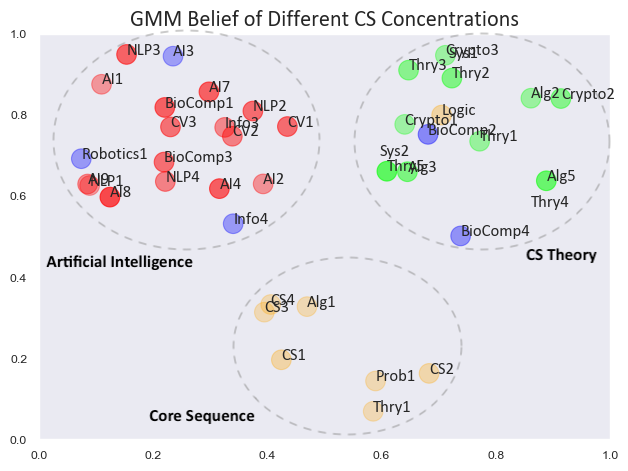
\includegraphics[scale=0.5]{figures/gmm_clusters.png}
    \caption{A visualization of the semantic meaning captured by the latent space of the model. Translucency corresponds to the count of students from the particular latent state, with more students leading to higher opacity.}
    \label{fig:gmm_clusters}
\end{figure}

\section{Applications}

In this section we present results from two different experiments performed with our proposed model. These applications demonstrate only a fraction of the model's scope, but show its power to provide insights.

\subsection{Quantifying Enrollment Likelihood}

One of the useful applications unique to our generative model is in quantifying enrollment likelihood. \nvg{These next few sentences should be improved} By training a model on a fraction of the enrollments and evaluating the likelihood of the held-out enrollments, we can get a sense of how unusual the held-out enrollments are by comparison. Taking this principle to its extreme, we can train a model for each student on every other student's enrollments, allowing us to model exactly how much each particular student varies from the typical. 

Figure~\ref{fig:likelihistogram} shows a histogram of the log-likelihood assigned to each undergraduate student in the computer science department using this process. The far left of the histogram contains students whose enrollments are highly atypical, and as we move right these students become less ``surprising" to the model. Most students fall within the middle range, making them neither highly unusual nor cookie-cutter.

By examining the classes taken by students who fall within each region of the histogram, we see that the model captures at least two meaningful axes of variance. Firstly, it recognizes that it is rare for students to take a very diverse set of courses spanning many academic subjects. This insight is shown in Figure~\ref{fig:piecharts}, which shows graphically the average coursework for each type of student. The second insight that the model captures is the spectrum of ambition. \nvg{Need more explanation of the next few sentences} More specifically, the model places very low probability on the small subgroup of students that take up to 30 computer science classes while placing high probability on just taking what is required within the department. On average atypical students take around 10 more courses than their counterparts. 

\begin{figure}
    \centering
    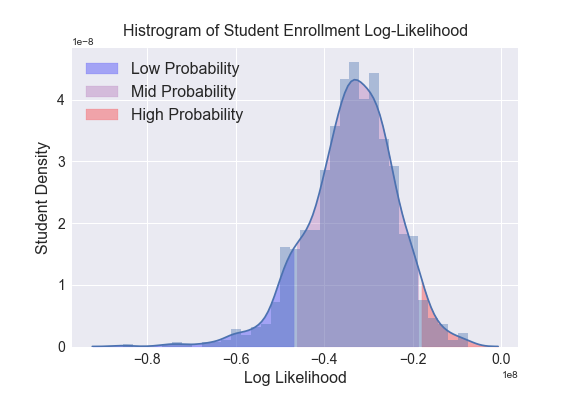
\includegraphics[scale=0.4]{figures/loglikelihood_hist.png}
    \caption{\label{fig:likelihistogram} Histogram of log-likelihoods for each student assigned by model trained on all other students. The three subpopulations of students discussed are highlighted in separate colors.}
\end{figure}

\begin{figure}[h]
    \centering
    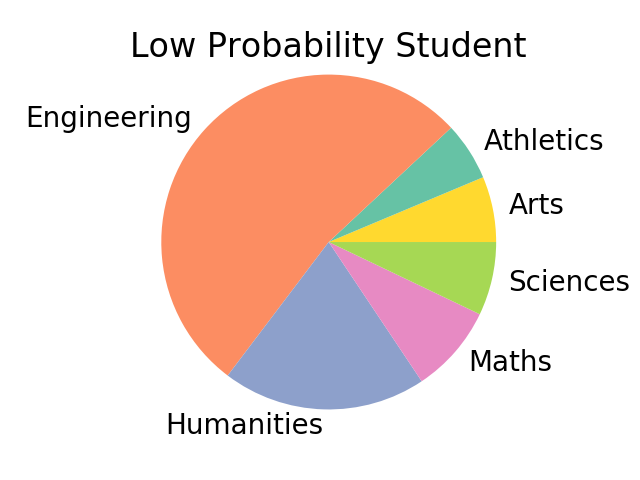
\includegraphics[scale=0.25]{figures/lowpie.png}
    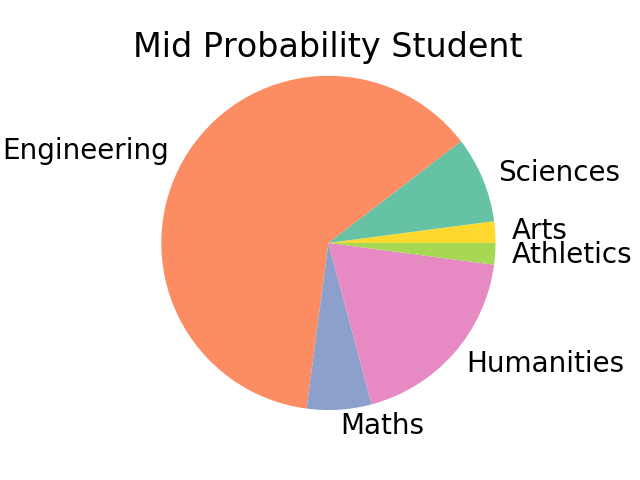
\includegraphics[scale=0.25]{figures/midpie.png} \\
    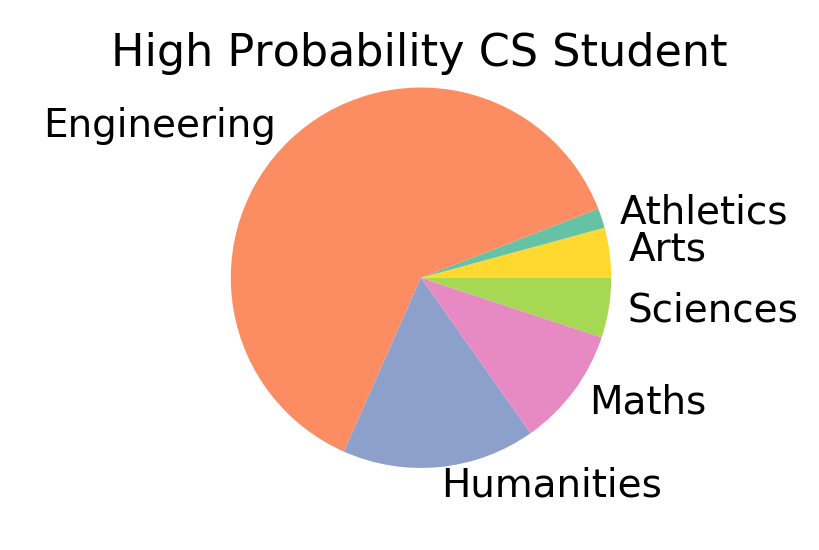
\includegraphics[scale=0.25]{figures/highpie.png}
    \caption{\label{fig:piecharts} Pie charts representing the difference between enrollment patterns captured by the model. Sections correspond to the average number of courses taken in a academic subject by the average student in the respective probability range.}
\end{figure}

\subsection{Understanding Paths}

   
\begin{figure*}[h!]
    \centering
    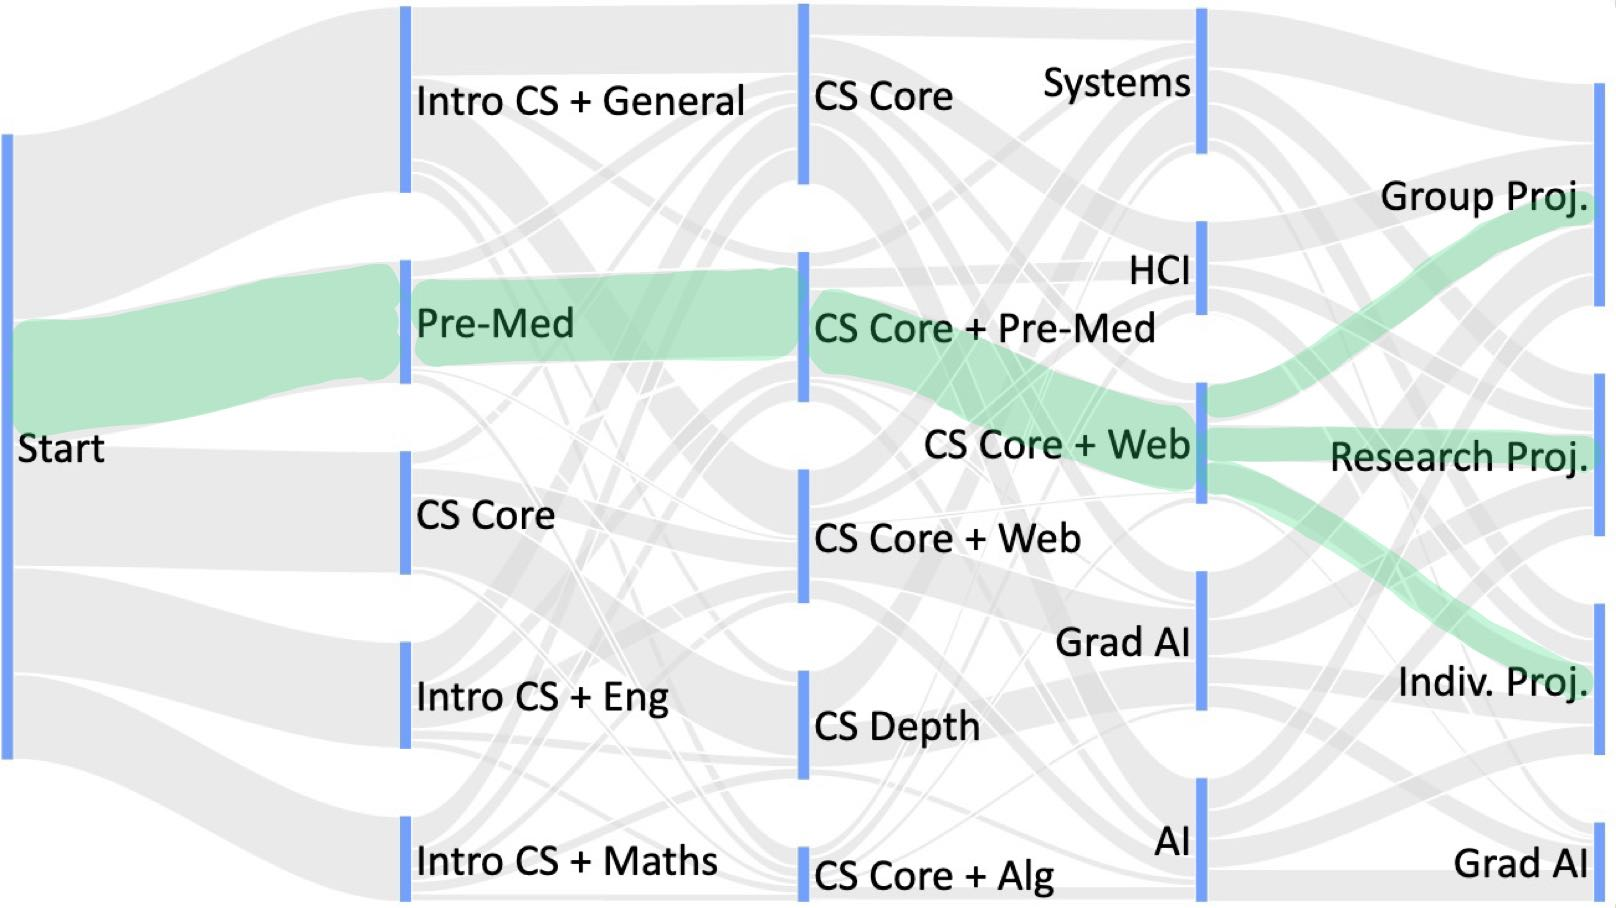
\includegraphics[width=0.45\linewidth]{figures/premed_highlight.jpg} 
    \qquad
    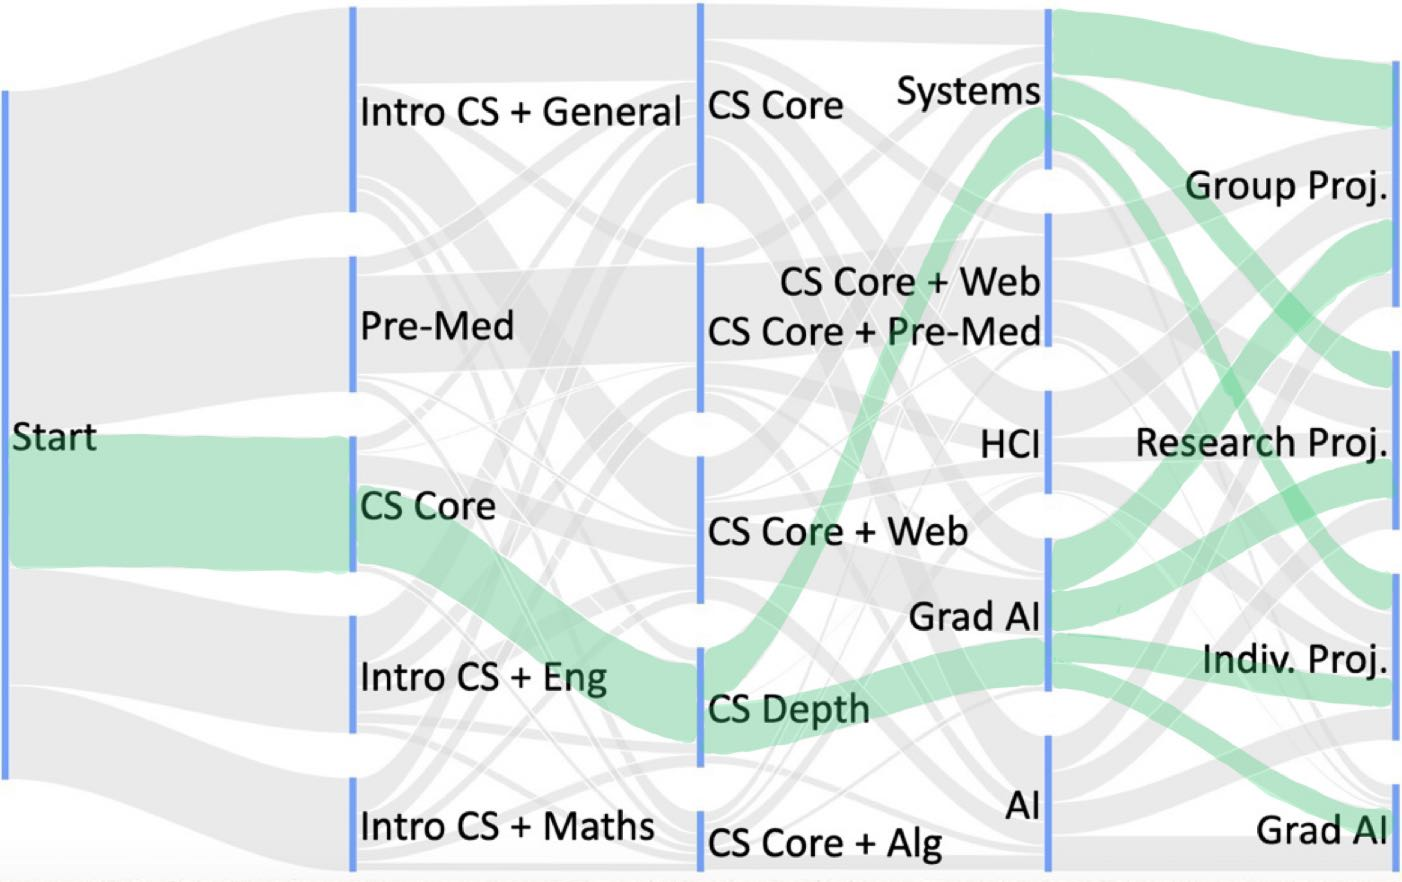
\includegraphics[width=0.41\linewidth]{figures/systems_highlight.jpg}
    % 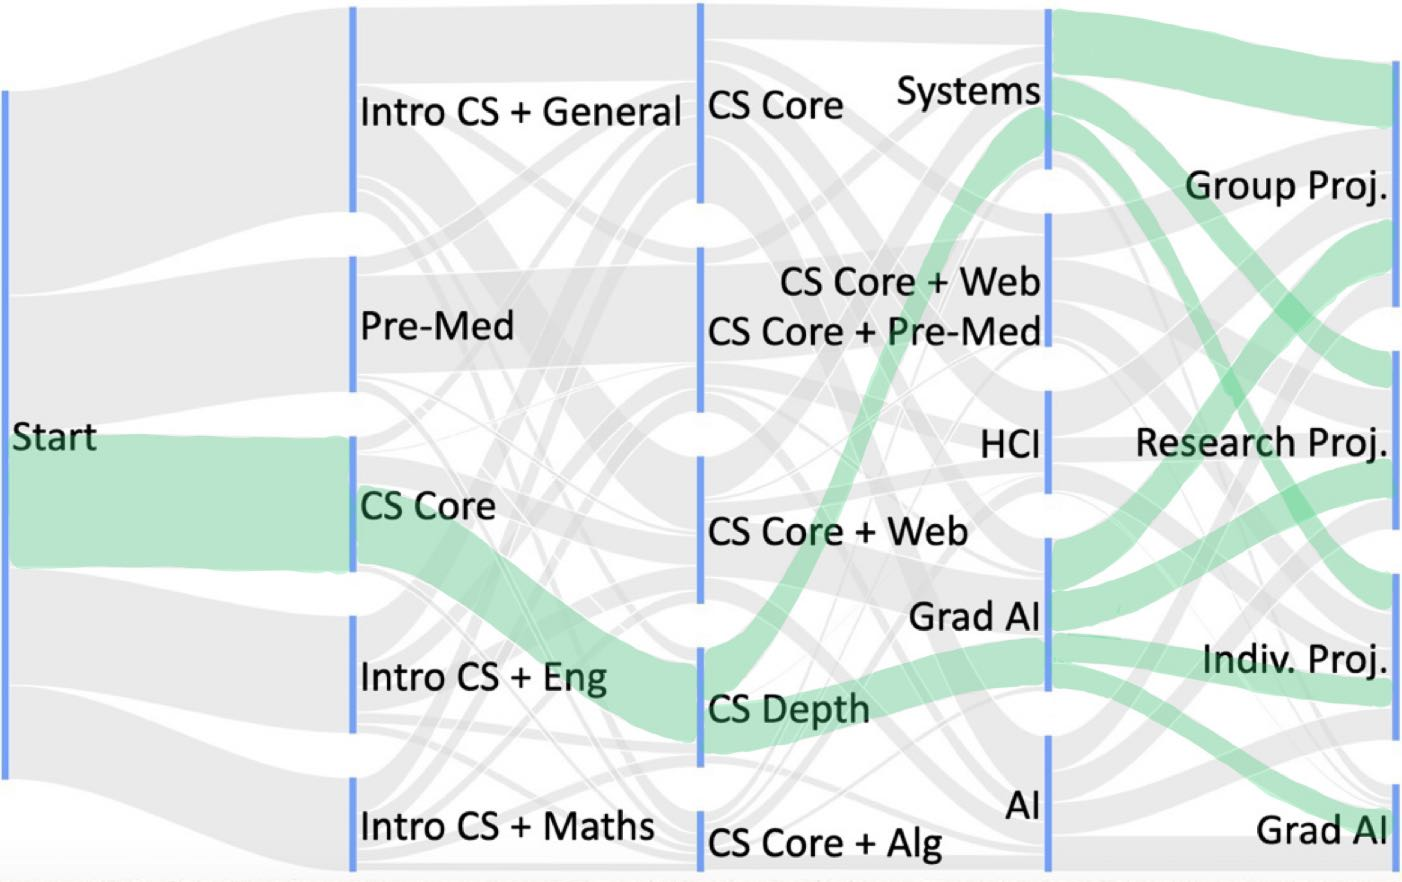
\includegraphics[width=0.48\linewidth]{figures/systems_highlight.png} 
    \caption{\label{fig:cs_sankeys} Two shadings of the same Sankey diagram constructed from the CMM trained on CS undergraduate enrollments. Top: A common path taken by students engaging in pre-med requirements is highlighted in blue. Bottom: A common path for students committed to in-depth study of computer science is highlighted.}
\end{figure*}

Perhaps the most unique capability of the model presented here is the ability to analyze sequences of enrollments, from inferring likely paths between X and Y, to uncovering unspoken student strategies. We can display this visually using Sankey diagrams in which the width of the line between adjacent segments is proportional to the transition probability between the corresponding hidden states in the model. Figures~\ref{fig:cs_sankeys} and \ref{fig:math_sankeys} show this style of Sankey for CS and Math students respectively.

Focusing specifically on Figures~\ref{fig:cs_sankeys}, we can note the two types of paths highlighted in the diagram. The first of these captures students who were actively taking the pre-medical requirements freshman and sophomore year. These same students were subsequently much more likely to take depth courses later and were more likely to focus on web development of information systems in their depth courses. We can contrast these students with the students that are highly committed to the CS major and its core classes starting freshman year. These students are much more likely to enroll in depth classes by their sophomore year and are predisposed towards the systems and AI concentrations within the major.
   
As a counterpoint, we can also examine Figure~\ref{fig:math_sankeys}, which shows an equivalent Sankey diagram for undergraduate students in mathematics. \nvg{Ali, wax poetic about math students here}


% \begin{figure}
    % \centering
    % 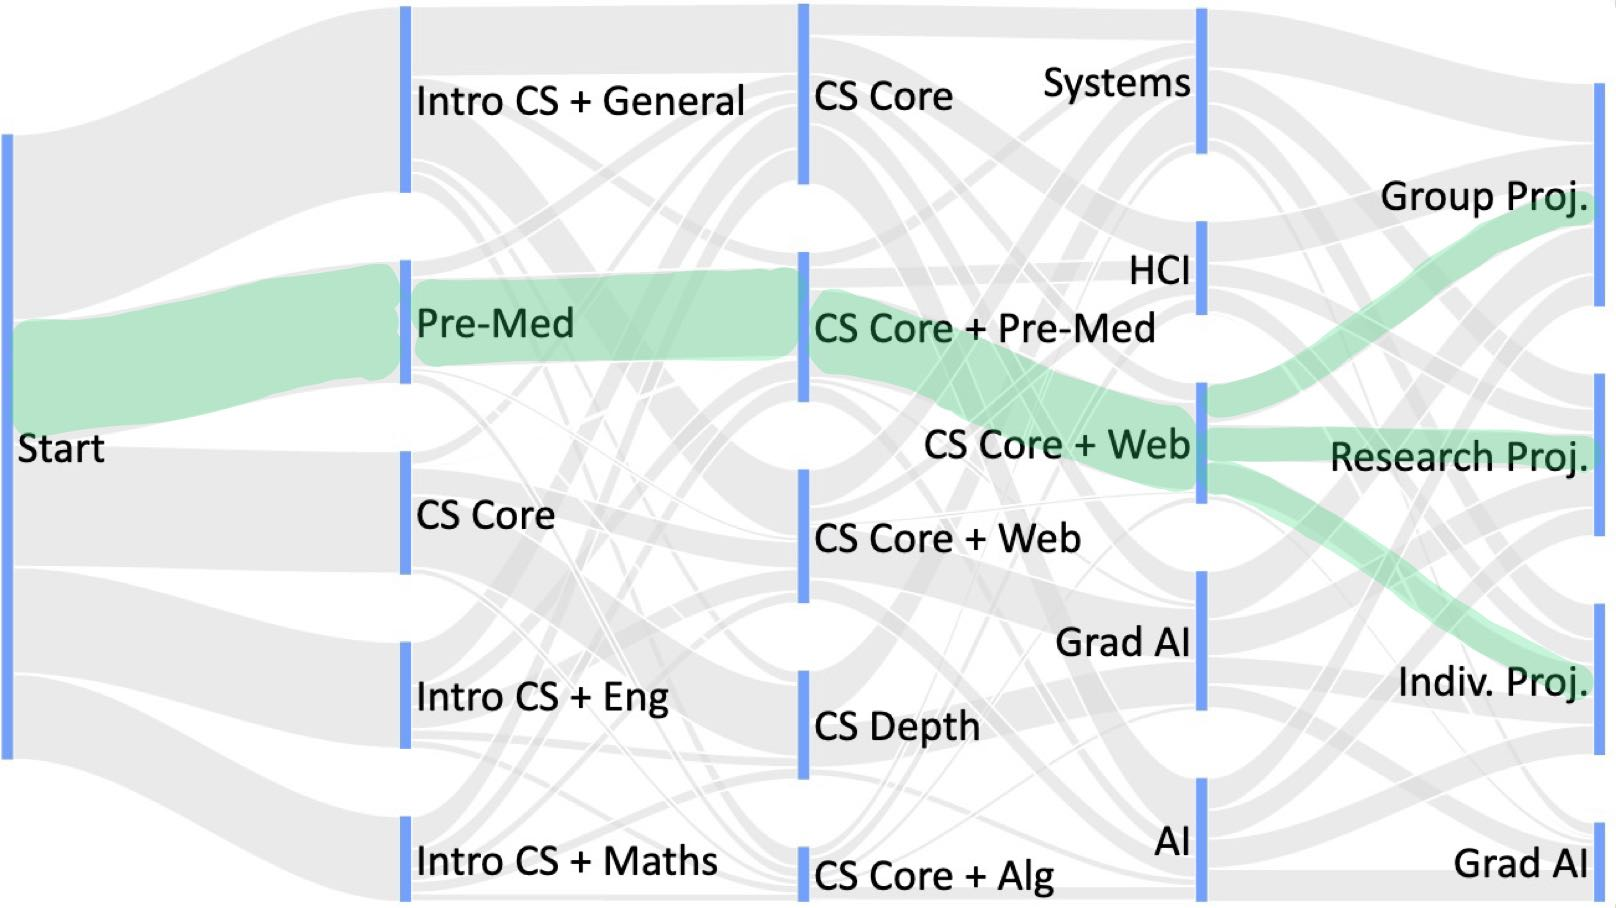
\includegraphics[scale=0.12]{figures/premed_highlight.png} \\
    % 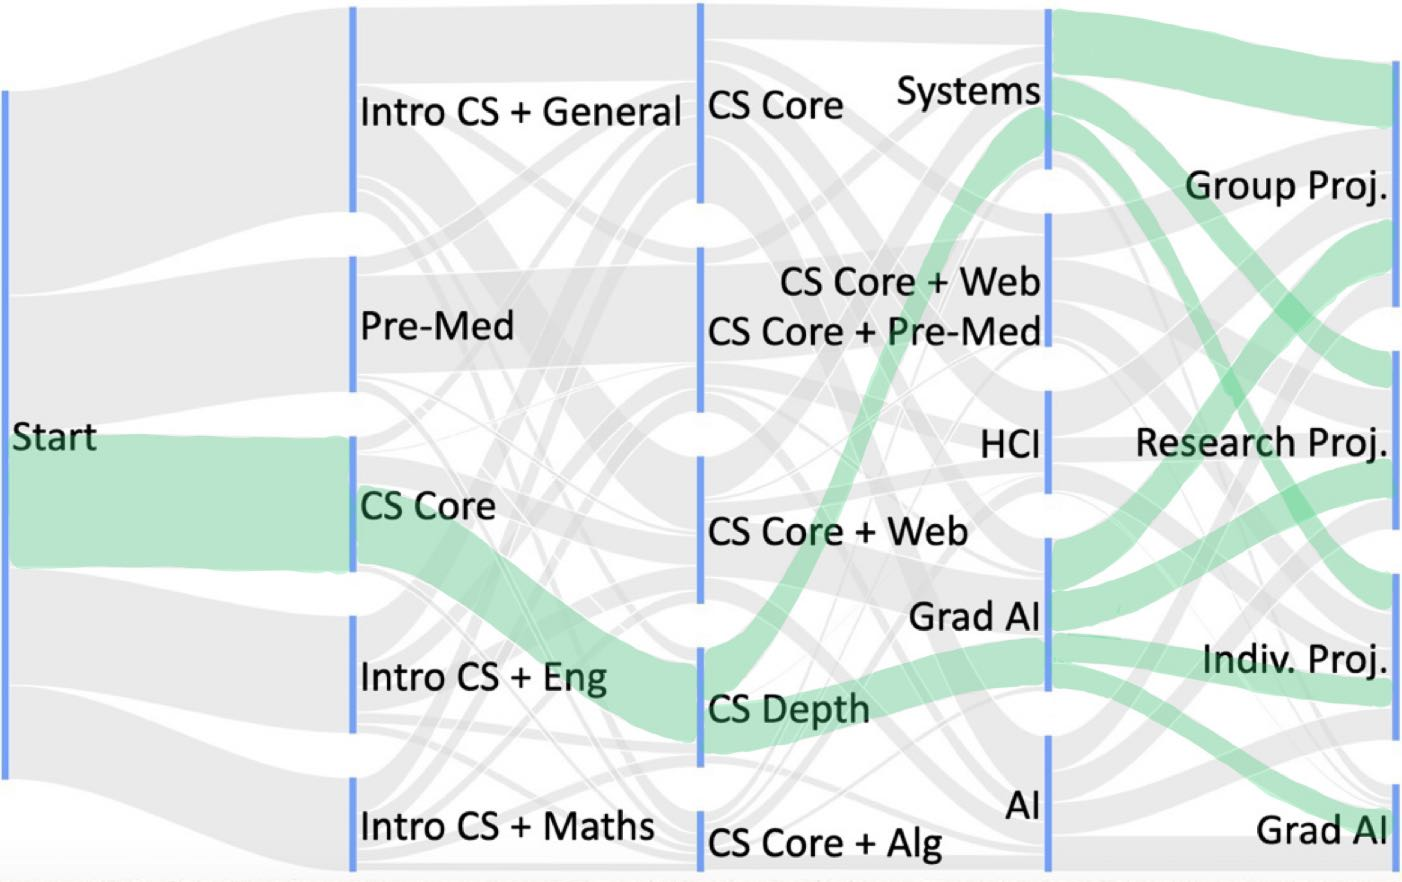
\includegraphics[scale=0.12]{figures/systems_highlight.png} 
    % \caption{\label{fig:math_sankeys} A placeholder holder Sankey diagram that will be replaced with one representing the transition probabilities in the contextual GMM.}
% \end{figure}
   
\section{Discussion}

So far we have presented a novel probabilistic model of enrollments, shown how to prove its soundness, and demonstrated how to use this model to perform novel educational research. The capabilities of this model are in most cases a superset of those offered by others, and the model can be trained easily with little intimate knowledge of the institution. 

There are, however, a noteworthy drawbacks of our approach. First among these is the strictly Markovian nature of the model. Though this assumption allows us to easily learn the parameters of the model, in practice the enrollments observed at one timestep will impact those sampled at the next timestep. These effects are to some extent modeled by the latent structure of the model, but an alternative approach, sacrificing the Markov assumption would capture more of these effects with a smaller number of hidden states. Our approach, on the other hand, is effective with less training data than, for example, a recurrent neural net, such as an LSTM. Our method is therefore more easily deployed for smaller institutions than ours.

Another limitation of the current work is the smoothing step we use to reduce the dimensionality of the data. Though in most cases this reduction is benign, it can in some cases erase patterns that exist in the data but which would only be measurable in aggregate across courses. Take for example the enrollment of engineering students in many different small humanities seminars. No individual seminar witnesses significant enrollments, but in aggregate they create a discernible pattern. Such effects can be ignored by a model that focuses on class enrollments on a per class basis, not per subject or department, as our does. This problem could be easily addressed by a hierarchical latent space that allows the model to learn aggregates trends across small groups of classes. One drawback of the increase in complexity, however, would be a corresponding decrease in interpretability. 

Lastly, we would like to note the potential for future work that links data we used here with other rich information sources such as demographic and grade data. Given that we were able to learn a semantically meaningful representation with enrollment data alone, it is easy to imagine how much more powerful the model could become with access to additional information sources--not only in its ability to recreate the empirical features of the distribution but also in the potential of the model to offer insights that are meaningful to students and staff. 

%ACKNOWLEDGMENTS are optional
\section{Acknowledgments}

We would like to acknowledge the support of the Stanford CartaLab, which offered guidance to us in our research.  

% The following two commands are all you need in the
% initial runs of your .tex file to
% produce the bibliography for the citations in your paper.
\bibliographystyle{abbrv}
\bibliography{sigproc} 

\balancecolumns
\appendix
\section{Contextual Mixture Model Details}
\subsection{EM Parameter Update}

\end{document}
